\documentclass[aps,prl,reprint,superscriptaddress,nofootinbib]{revtex4-2}
\usepackage{amsmath,amssymb,bm,graphicx,booktabs}
\usepackage[hidelinks]{hyperref}
\usepackage{orcidlink}
\newcommand{\R}{\mathbb R}
\newcommand{\C}{\mathbb C}
\newcommand{\rank}{\operatorname{rank}}
\newcommand{\Tr}{\operatorname{Tr}}
\newcommand{\full}{\mathrm{full}}
\newcommand{\obs}{\mathrm{obs}}
\newcommand{\cert}{\mathrm{cert}}
\newcommand{\PT}{\mathrm{PT}}
\newcommand{\bigO}{\mathsf O}
\begin{document}

\title{Single-Slot Tomography Cannot Self-Certify Multitime Response Dimension}
\author{Yongzi Chen\,\orcidlink{0009-0008-6202-002X}}
\email{23103646d@connect.polyu.hk}
\affiliation{Department of Physics and Materials, The Hong Kong Polytechnic University, Hung Hom, Hong Kong, China}

\begin{abstract}
Can finite experiments certify that the response directions they have observed exhaust those accessible to every registered multitime protocol?  For single-slot tomography---experiments that intervene at one time while resetting the rest---the answer is no: we exhibit a two-qubit collision model whose complete single-slot data are unchanged by a smooth, non-gauge memory rotation that a retained two-time correlator detects at first order, and a delayed-chain family in which an arbitrarily clean finite Hankel plateau is false at every tested horizon.  Certification becomes possible relative to an externally justified response-order bound $n_J$: a rank-saturated flat response core then determines every registered value and first derivative at arbitrary depth, and finite data return certified-within-class, class-excluded, or inconclusive verdicts.  Sealed runs on two IBM processors reproduced all planted signals; an unreferenced absolute threshold lost specificity on one processor, and a preregistered device-referenced differential test on that processor then detected all planted directions with zero null false positives.
\end{abstract}
\maketitle

\paragraph{The question.---}
A process tensor is fixed by an informationally complete intervention basis, whereas restricted controls determine only a restricted multitime object~\cite{Pollock2018ProcessTensor,White2020ProcessControl,White2022ProcessTomography,Giarmatzi2025Multitime}.  Restricted unitary sequences can still witness selected multitime properties~\cite{White2025UnitarySequences}, and quantum Markov order depends on the conditioning instrument~\cite{Taranto2019MarkovOrder}.  We call a causal-break experiment \emph{single slot} when it probes one time and resets or discards the remaining ports.  Can a finite family of such experiments certify that its derivative kernel already equals the kernel of every protocol generated by a declared intervention algebra?  Equivalently, can it certify the dimension of the minimal smooth response model, rather than a Hilbert-space dimension~\cite{Brunner2008,Gallego2010}?  The answer is no without an explicit closure condition.

\paragraph{Proposition 1: exact single-slot blindness.---}
Consider registers $[S_1,E,S_2]$, initialize $E$ in $|+\rangle$, and apply
\begin{equation}
 U_\delta=CZ_{S_2E}\,R_x^E(\delta)\,CZ_{S_1E},
 \qquad R_x(\delta)=e^{-i\delta X/2},
 \label{eq:comb}
\end{equation}
followed by discarding $E$.  At either slot, prepare one of the six Pauli eigenstates, measure a binary Pauli POVM, and close the other slot by a causal break feeding $I/2$.  The resulting 48 coordinates span the preparation and readout spaces of each marginal qubit channel.

Every slot-1 statistic is independent of $\delta$, because all $\delta$-dependent operations occur downstream on $ES_2$ and are trace preserving there.  For slot 2,
\begin{equation}
 \Tr_{S_1}\!\left[CZ\left(I/2\otimes|+\rangle\!\langle+|\right)CZ\right]=I_E/2,
 \label{eq:pinning}
\end{equation}
which is fixed by every unitary link.  Thus all single-slot probabilities agree on the entire link family, not merely to first order.  Retaining both system outputs changes the verdict: for $S_1=S_2=|+\rangle$,
\begin{equation}
 \langle Y_{S_1}X_{S_2}\rangle_\delta=\sin\delta,
 \qquad \left.\partial_\delta\right|_0=1.
 \label{eq:separator}
\end{equation}
The induced $S_1S_2$ channel has Choi rank two for every $SU(2)$ link, so one memory qubit is a minimal Stinespring environment.  Left multiplication by $R_z$ is an exact gauge only relative to the registered system-port algebra: it commutes through the fixed $Z$-diagonal couplings and disappears under $\Tr_E$.  At the identity the quotient link tangent is spanned by $X_E,Y_E$; its single-slot response rank is zero and its full registered response rank is two.

This is the annihilator geometry of an incomplete multitime tester span, not a new failure of process-tensor tomography; its sharp content is exact all-parameter agreement, complete marginal-channel tomography, a minimal dilation, and a non-gauge first-order separator, distinct from Hamiltonian identifiability through one fixed probe~\cite{SoneCappellaro2017}.

\begin{figure*}[t]
 \centering
 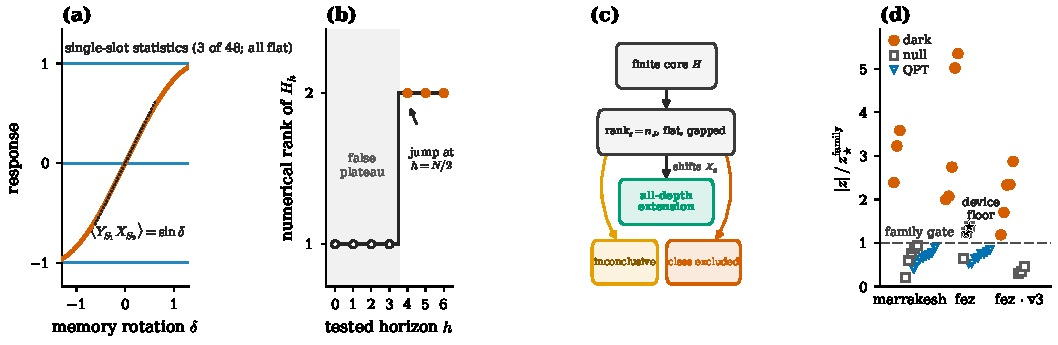
\includegraphics[width=0.98\textwidth]{figures/c7_flat_extension.pdf}
 \caption{Non-self-certification and its order-conditioned repair.  (a) Single-slot causal-break statistics of the $CZ$--$R_x(\delta)$--$CZ$ comb are exactly constant in $\delta$ (three of 48 shown, blue), while the retained two-slot correlator $\langle Y_{S_1}X_{S_2}\rangle=\sin\delta$ (vermillion) has unit slope at the working point.  (b) Numerical rank of the first-jet Hankel matrix $H_h$ versus tested horizon $h$ for a delayed hidden chain ($N=8$): the rank-one plateau over $h<N/2$ is arbitrarily clean yet false, so a stable plateau alone is never a pass.  (c) Certification pipeline: a finite core passing rank saturation ($\mathrm{rank}_\varepsilon=n_J$), two-sided flatness, and gap margin yields the unique exact all-depth extension via the shifts $X_a$ (green); on noisy data the audit instead returns \textsc{inconclusive} (amber) or excludes the declared class (vermillion).  (d) Sealed hardware instances, $|z|$ normalized by each decision family's frozen gate $z_\star^{\mathrm{family}}$ so the unit line is the common pass/fail boundary: planted darks (vermillion) versus nulls (grey) on \texttt{ibm\_marrakesh}, \texttt{ibm\_fez}, and the device-referenced differential rerun (fez\,$\cdot$\,v3); marginal-tomography controls (QPT, blue) stay below their gate throughout ($0/16$).  The starred fez nulls are the device-locked floor that motivated v3 ($5/5$ darks, $0/3$ nulls).}
 \label{fig:flat}
\end{figure*}

\paragraph{Why a finite plateau is insufficient.---}
For any tested prefix/suffix horizon $h$, take the direct sum of a one-dimensional visible process and a hidden classical chain $e_0\to e_1\to\cdots\to e_N$ with $N>2h+2$.  Let the last transition depend smoothly on $\theta$ and let the final effect see only $e_N$.  Every measured zeroth- and first-order Hankel entry below that horizon equals the visible rank-one data and can have an arbitrarily clean singular gap; a new derivative appears only at depth $N$.  This diagonal CPTP family proves that no fixed number of flat steps establishes all-depth closure.

\paragraph{Relation to realization and spectral learning.---}
Finite Hankel rank and spectral factorization are classical tools in stochastic realization~\cite{CarlylePaz1971,ArbibManes1980} and in spectral learning of hidden Markov models, predictive-state representations, and weighted automata~\cite{Hsu2012HMM,Boots2011PSR,BalleMohri2012WFA,Balle2014WFA,BalleMohri2018WFA}.  In the quantum setting, block-Hankel process identification already establishes the finite-duration principle for a fixed repeatedly applied channel: finite records alone cannot certify completeness, but an effective-dimension upper bound restores it through Ho--Kalman reconstruction~\cite{BenninkLougovski2019QPI}; completely positive realization and passive-system identification appear in Refs.~\cite{MonrasWinter2016,GutaYamamoto2016}.  We extend this framework to word-indexed first-jet response series generated by multi-letter intermediate interventions, obtaining exact non-gauge blindness under complete marginal tomography, the complete response kernel of a declared intervention algebra, three-state finite-data certificates, and a sealed device-referenced hardware protocol.  ``Flat extension'' here means closure of response-Hankel row and column spaces under registered shifts; it is unrelated to positivity and representing measures in the Curto--Fialkow moment problem~\cite{CurtoFialkow1998}.

\paragraph{Saturated first-derivative extension.---}
Let $\Sigma$ be a finite ordered alphabet of $m$ unnormalized CP branches; intrinsic links and finite-controller phases are included in the letter labels.  At a working point $x_0$, lift each letter to
\begin{equation}
 \bm A_a=
 \begin{pmatrix}
 A_a^0&0\\ D_a&I\otimes A_a^0
 \end{pmatrix},
 \label{eq:jetlift}
\end{equation}
with preparation and readout derivatives at the boundaries.  Multiplication of these block-triangular matrices is the chain rule and sums the differentiated insertion over every occurrence in a word.  Stack values and tangent-coordinate derivatives into a response series $y_{\lambda i}(w)$.  The declared class $\mathcal C(n_J)$ consists of series whose minimal reachable/observable linear realization has order at most $n_J$.  This upper bound is external input: for example, a verified finite controller and a separately bounded accessible memory carrier imply $n_J\le(1+p)d_{\rm acc}$ for $p$ tangent coordinates.

A \emph{saturated flat core} is a finite block of $y$ over prefix and suffix sets $\mathcal P,\mathcal S$ whose Hankel matrix $H$ reaches rank $n_J$ and whose row and column spaces are closed on both sides under every registered one-letter shift and boundary vector [Eqs.~(\ref{eq:hankel})--(\ref{eq:flat}), End Matter].

\textit{Order-conditioned closure theorem.}---Every $y\in\mathcal C(n_J)$ consistent with a saturated flat core has the unique all-depth extension
\begin{equation}
 \boxed{\ y_{\lambda i}(w)=\widehat f_\lambda X_w\widehat s_i
 \quad\forall w\in\Sigma^*\ },
 \label{eq:extension}
\end{equation}
up to simultaneous similarity, where the shifts $X_a$ and boundary vectors $\widehat f_\lambda,\widehat s_i$ are compressions of the core [Eq.~(\ref{eq:reconstruction}), End Matter].

The proof has four steps (End Matter; complete lemma chain in the Supplemental Material~\cite{SupplementalMaterial}).  The infinite response-Hankel matrix has rank equal to the minimal realization order $n(y)$, and $\rank H\le n(y)\le n_J$, so a core reaching $n_J$ already exhausts the infinite rank.  Two-sided flatness makes every registered one-letter shift a well-defined operator on the $n_J$-dimensional core quotient.  Products of these shifts are then forced to reproduce the response of every word.  Uniqueness follows because any two rank factorizations of the same core are related by the similarity that intertwines the reconstructions.

The reconstruction is isomorphic to the reachable/observable part of every physical first-derivative realization and gives
\begin{equation}
 K_{\full}^{\mathcal I}=
 \bigcap_{w,b,i}\ker dp_{bi}(w;x_0),
 \label{eq:kernel}
\end{equation}
where $\mathcal I$ labels the declared intervention algebra.  The superscript in $d_{\rm op}^{(1)}=\dim T_{x_0}M-\dim K_{\full}^{\mathcal I}$ labels first derivative order.  Finite randomization, summed outcome branches, and finite classical feed-forward either enlarge the finite controller alphabet or form finite linear combinations of word probabilities.  Their derivatives obey the same combinations, so Eq.~\eqref{eq:kernel} is also the kernel of every protocol generated by $\mathcal I$; direct access to an undeclared environment remains outside the class.

\paragraph{Finite-data certificate.---}
Finite precision never proves that a small singular value is exactly zero, so the audit returns one of three preregistered verdicts.  \textsc{Certified}: rank saturation at $n_J$, two-sided flatness residuals, and spectral-gap margins all pass within certified error budgets, and the extension holds within the declared class.  \textsc{Rejected}: an $(n_J{+}1)$-th response direction or a closure violation is resolved above its stated threshold, excluding the declared class itself.  \textsc{Inconclusive}: anything else---an unresolved gap, an uncertified factor alignment, or a missing rank promise.  The quantitative gap, subspace-angle, and truncation bounds behind these verdicts are collected in End Matter [Eqs.~(\ref{eq:theoremP})--(\ref{eq:truncated-core-main})].

\paragraph{Entry and sampling resources.---}
With supplied or independently certified saturated bases, the certificate uses $O(mn_J^2)$ response entries at word depth at most $2n_J-1$, whereas unrestricted depth-$k$, $d$-level comb tomography must resolve a $\Theta(d^{4k})$-dimensional affine set [Eqs.~(\ref{eq:entries})--(\ref{eq:comb-dim}), End Matter].  The scaling counts response entries; shot complexity is set separately by the requested precision and confidence, with an explicit Hoeffding upper bound in the Supplemental Material~\cite{SupplementalMaterial}.

\paragraph{Sealed hardware tests.---}
On \texttt{ibm\_marrakesh}, a sealed eight-instance run detected all $3/3$ planted directions with $0/5$ null false positives, and matched single-slot tomography detected $0/3$, as Proposition 1 predicts.  On \texttt{ibm\_fez}, the same frozen estimator detected all $5/5$ planted directions and single-slot tomography again detected $0/5$, but $2/3$ nulls crossed the unreferenced absolute gate; a separately sealed six-null confirmation found a reproducible negative $YX$ floor (pooled $z=-6.20$) on one deterministic physical layout, consistent with a device-locked readout bias rather than a planted memory link.  A preregistered device-referenced differential test on the affected processor then detected $5/5$ planted directions with $0/3$ null false positives.  Sensitivity transferred across devices; specificity of an absolute threshold did not, and the audit's reference discipline caught it.  These runs stress-test the blind-direction obstruction, separator sensitivity, and reference calibration of the audit; the order bound and the saturated basis enter as declared external inputs, exactly as in the theorem.  Power planning, shot budgets, and complete run manifests are in the Supplemental Material~\cite{SupplementalMaterial}.

\paragraph{Outlook.---}
The result converts a structural impossibility into a conditional experimental discipline: single-slot completeness is not assumed, all-depth closure is asserted only after an independently justified order bound is saturated, and unresolved evidence returns inconclusive.  Open problems are blind basis discovery, experimentally independent order bounds, higher derivative orders, and cross-vendor validation with device-referenced controls.

\paragraph{Data availability.---}
The data and software supporting this study---including IBM job outputs, calibration snapshots, sealed manifests, verification hashes, analysis code, and manuscript-generation scripts---are openly available in the public repository release \texttt{v1.0} at \url{https://github.com/ccyyyYyzz/flat-extension-certificate/releases/tag/v1.0}.

\begin{acknowledgments}
The author acknowledges use of IBM Quantum services.  The views expressed are those of the author and do not reflect the official policy or position of IBM or the IBM Quantum team.
\end{acknowledgments}

\bibliography{references}

\section*{End Matter}

\setcounter{equation}{0}
\renewcommand{\theequation}{A\arabic{equation}}
\paragraph{Appendix A: saturated core and proof summary.---}
\label{app:core}
For finite prefix and suffix sets $\mathcal P,\mathcal S$, define
\begin{align}
 H_{(\lambda,s),(i,p)}&=y_{\lambda i}(sp),&
 (H_a)_{(\lambda,s),(i,p)}&=y_{\lambda i}(sap),\nonumber\\
 (c_i)_{(\lambda,s)}&=y_{\lambda i}(s),&
 (r_\lambda)_{(i,p)}&=y_{\lambda i}(p).
 \label{eq:hankel}
\end{align}
Write a rank factorization $H=OR$, where $O$ and $R$ are observability and reachability factors (unrelated to the rotation $R_x$ or the asymptotic symbol $\mathsf O$).  A saturated flat core obeys, for every $a$,
\begin{equation}
 \begin{aligned}
 \rank H&=n_J,\\
 (I-OO^\dagger)H_a&=0,
 &H_a(I-R^\dagger R)&=0,\\
 (I-OO^\dagger)c_i&=0,
 &r_\lambda(I-R^\dagger R)&=0.
 \end{aligned}
 \label{eq:flat}
\end{equation}
Choose $O^LO=I$ and $RR^R=I$ and set
\begin{align}
 X_a&=O^LH_aR^R,\nonumber\\
 \widehat s_i&=O^Lc_i,
 &\widehat f_\lambda&=r_\lambda R^R.
 \label{eq:reconstruction}
\end{align}
Flatness guarantees that every one-letter continuation of core data stays inside the spans factored by $O$ and $R$, so the compressions in Eq.~\eqref{eq:reconstruction} lose nothing at any depth, and induction over word length yields Eq.~\eqref{eq:extension}.  Any two rank factorizations of the same core are related by an invertible similarity that intertwines the reconstructed triples, which gives uniqueness.  The complete lemma chain, the invariant zero-order-unobservable filtration, and the cocycle bookkeeping are in the Supplemental Material~\cite{SupplementalMaterial}.

\setcounter{equation}{0}
\renewcommand{\theequation}{B\arabic{equation}}
\paragraph{Appendix B: finite-error verdicts and resources.---}
\label{app:errors}
For each response matrix $J_j$, $j\in\{A,F\}$, one of two preregistered specifications is used: either its exact rank $r_j$ is an independent structural promise of the declared model class, or a resolution $\tau_j>0$ is fixed and the observed spectrum obeys $\widehat\sigma_{r_j}>\tau_j+\varepsilon_j$ and $\widehat\sigma_{r_j+1}<\tau_j-\varepsilon_j$.  Let $\mathcal L_j$ be the corresponding declared-rank or $\tau_j$-resolved low-singular right subspace and $\widehat{\mathcal L}_j$ its observed counterpart.  With
\begin{align}
 \Delta_j&=\widehat\sigma_{r_j}-\widehat\sigma_{r_j+1}-\varepsilon_j,
 &b_j&=\min\!\left\{1,\frac{\varepsilon_j}{\Delta_j}\right\},\nonumber\\
 \eta_{\cert}&=\|P_{\widehat{\mathcal L}_A}-P_{\widehat{\mathcal L}_F}\|+b_A+b_F,
 \label{eq:theoremP}
\end{align}
Wedin's theorem~\cite{Wedin1972} gives
$\|P_{\mathcal L_A}-P_{\mathcal L_F}\|\le\eta_{\cert}$ when both gaps are positive.  This is a bounded-angle statement at a declared dimension or stated resolution; only an external exact-rank promise identifies $\mathcal L_j$ with a kernel.  Without such a promise or a clean threshold band, the subspace verdict is \textsc{inconclusive}.

For the noisy Hankel core, let $\widehat H_{n_J}$ be the rank-$n_J$ truncated SVD of the generally full-rank observation $\widehat H$.  The exact core obeys
\begin{equation}
 \|\widehat H_{n_J}-H\|
 \le\widehat\sigma_{n_J+1}+\varepsilon_H
 =:\overline\varepsilon_H.
 \label{eq:truncated-core-main}
\end{equation}
All coordinate-level shift, seed, readout, and prediction bounds must use factor-alignment radii certified on this full truncation ball; without an independently certified alignment, the audit retains only coordinate-free singular-subspace and closure-residual bounds.

Given supplied or independently certified saturated prefix and suffix bases, the core, its $m$ central shifts, and boundary data use at most
\begin{equation}
 N_{\rm flat}\le(m+1)n_J^2+(|I|+|\Lambda|)n_J
 \label{eq:entries}
\end{equation}
entries at depth at most $2n_J-1$.  The real affine dimension of an unrestricted depth-$k$, $d$-level comb is
\begin{equation}
 D_k=\frac{d^2(d^{4k}-1)}{d^2+1}=\Theta(d^{4k}),
 \label{eq:comb-dim}
\end{equation}
and any continuous scalar-coordinate tomography that is locally injective on a relative-interior neighborhood of the comb set requires at least $D_k$ independent scalar coordinates.  A bounded jet-entry oracle yields the explicit Hoeffding shot upper bound of the Supplemental Material~\cite{SupplementalMaterial}, where the matched-order comparator analysis is also recorded.

\end{document}
